\documentclass[11pt,a4paper]{article}
\usepackage[utf8]{inputenc}
\usepackage[french]{babel}
\usepackage[T1]{fontenc}

\usepackage{amsmath}
\usepackage{amsfonts}
\usepackage{amssymb}

\newcommand{\NomAuteur}{Fabrice BOISSIER}
\newcommand{\TitreMatiere}{Architecture des Ordinateurs 1}
\newcommand{\NomUniv}{EPITA - Bachelor Cyber Sécurité}
\newcommand{\NiveauUniv}{CYBER1}
\newcommand{\NumGroupe}{CYBER1}
\newcommand{\AnneeUniv}{2024-2025}
\newcommand{\DateExam}{juin 2025}
\newcommand{\TypeExam}{Rattrapage}
\newcommand{\TitreExam}{\TitreMatiere}
\newcommand{\DureeExam}{2h00}
\newcommand{\MyWaterMark}{\AnneeUniv} % Watermark de protection

% Ajout de mes classes & definitions
\usepackage{MetalExam} % Appelle un .sty

% "Tableau" et pas "Table"
\addto\captionsfrench{\def\tablename{Tableau}}

%%%%%%%%%%%%%%%%%%%%%%%
%Header
%%%%%%%%%%%%%%%%%%%%%%%
\lhead{\TypeExam}							%Gauche Haut
\chead{\NomUniv}							%Centre Haut
\rhead{\NumGroupe}							%Droite Haut
\lfoot{\DateExam}							%Gauche Bas
\cfoot{\thepage{} / \pageref*{LastPage}}	%Centre Bas
\rfoot{\texttt{\TitreMatiere}}				%Droite Bas

%%%%%

\usepackage{tabularx}

\newlength{\LabelWidth}%
%\setlength{\LabelWidth}{1.3in}%
\setlength{\LabelWidth}{1cm}%
%\settowidth{\LabelWidth}{Employee E-mail:}%  Specify the widest text here.

% Optional first parameter here specifies the alignment of
% the text within the \makebox.  Default is [l] for left
% alignment. Other options are [r] and [c] for right and center
\newcommand*{\AdjustSize}[2][l]{\makebox[\LabelWidth][#1]{#2}}%


\definecolor{mGreen}{rgb}{0,0.6,0}
\definecolor{mGray}{rgb}{0.5,0.5,0.5}
\definecolor{mPurple}{rgb}{0.58,0,0.82}
\definecolor{backgroundColour}{rgb}{0.95,0.95,0.92}

\lstdefinestyle{CStyle}{
    backgroundcolor=\color{backgroundColour},
    commentstyle=\color{mGreen},
    keywordstyle=\color{magenta},
    numberstyle=\tiny\color{mGray},
    stringstyle=\color{mPurple},
    basicstyle=\footnotesize,
    breakatwhitespace=false,
    breaklines=true,
    captionpos=b,
    keepspaces=true,
    numbers=left,
    numbersep=5pt,
    showspaces=false,
    showstringspaces=false,
    showtabs=false,
    tabsize=2,
    language=C
}


\hyphenation{op-tical net-works SIGKILL}


\begin{document}

\MakeExamTitleDuree     % Pour afficher la duree
%\MakeExamTitle                   % Ne pas afficher la duree

%% \MakeStudentName    %% A reutiliser sur chaque nouvelle page

\bigskip
%\bigskip

Vous devez respecter les consignes suivantes, sous peine de 0 :

\begin{table}[ht!]
  \begin{minipage}{0.45\textwidth}

\begin{enumerate}[label=\Roman*)]
\item Lisez le sujet en entier avec attention
\item Répondez sur le sujet
\item Ne trichez pas
\item Ne détachez pas les agrafes du sujet
\end{enumerate}

  \end{minipage}
  \hfillx
  \begin{minipage}{0.55\textwidth}

\begin{enumerate}[label=\Roman*),start=5]
\item \'Ecrivez lisiblement vos réponses (si nécessaire en majuscules)
\item Les appareils électroniques sont tous interdits (calculatrices également)
\end{enumerate}

  \end{minipage}
\end{table}


%\begin{itemize}
%\item Lisez le sujet en entier avec attention
%\item Répondez sur le sujet
%\item Ne détachez pas les agrafes du sujet
%\item \'Ecrivez lisiblement vos réponses (si nécessaire en majuscules)
%\item Les appareils électroniques sont tous interdits (calculatrices également)
%\item Ne trichez pas
%\end{itemize}

%\bigskip

%\vfillFirst

% Questions cours
\section{Conversions (10 points)}

\subsection{(2 points) Rappelez les 14 premières puissances de 2 : }

\medskip


\begin{table}[ht!]
\centerline{
\begin{tabular}{ | m{0.5cm} | m{0.5cm} | m{0.5cm} | m{0.5cm} | m{0.65cm} | m{0.65cm} | m{0.65cm} | m{1cm} | m{1cm} | m{1cm} | m{1.5cm} | m{1.5cm} | m{1.5cm} | m{1.5cm} |}
\hline
$ 2^{0} $ & $ 2^{1} $ & $ 2^{2} $ & $ 2^{3} $ & $ 2^{4} $ & $ 2^{5} $ & $ 2^{6} $ & $ 2^{7} $ & $ 2^{8} $ & $ 2^{9} $ & $ 2^{10} $ & $ 2^{11} $ &  $ 2^{12} $ &  $ 2^{13} $ \\
\hline
 & & & & & & & & & & & & & \\
 & & & & & & & & & & & & & \\
 & & & & & & & & & & & & & \\
\hline
\end{tabular}
}
\end{table}


%\bigskip

%%%%%%%%%%%%%%%%%%%%%%%%%%%%%%%%%%


\subsection{(2 points) Convertissez ces nombres en décimaux. Vous donnerez leur interprétation non-signée puis signée sur 12 bits.}

\medskip

\centerline{
\begin{tabular}{ c ||  C{6cm} || C{6cm} }
 & \multirow{3}{*}[0pt]{non-signé}
 & \multirow{3}{*}[0pt]{signé}
 \\
%
 & & \\
 & & \\
%
\hline
\multirow{3}{*}[0pt]{ $ \% \, 0101 \; 1010 \; 0101 $ } & & \\
 & & \\
 & & \\
\hline
\multirow{3}{*}[0pt]{ $ \% \, 1010 \; 1011 \; 1010 $ } & & \\
 & & \\
 & & \\
\hline
\multirow{3}{*}[0pt]{ \$ 7AB } & & \\
 & & \\
 & & \\
\hline
\multirow{3}{*}[0pt]{ \$ B95 } & & \\
 & & \\
 & & \\
\end{tabular}
}

\bigskip

%%%%%%%%%%%%%%%%%%%%%%%%%%%%%%%%%%

\subsection{(2 points) Convertissez ces nombres décimaux en binaire sur 12 bits, puis en hexadécimal.}

\medskip

\centerline{
\begin{tabular}{| c ||c|| c ||C{0.33cm}|C{0.33cm}|C{0.33cm}|C{0.33cm} || C{0.33cm}|C{0.33cm}|C{0.33cm}|C{0.33cm} || C{0.33cm}|C{0.33cm}|C{0.33cm}|C{0.33cm} ||c|| c ||C{0.33cm}|C{0.33cm}|C{0.33cm}| }
\hline
                   & & \multicolumn{13}{c||}{\multirow{2}{*}{binaire}}  & & \multicolumn{4}{c|}{\multirow{2}{*}{hexadécimal}} \\
                   & & \multicolumn{13}{c||}{ }                         & & \multicolumn{4}{c|}{ }                            \\
\hline
\multirow{2}{*}{$ 1592 $} & \cellcolor{black!45} &
  \multirow{2}{*}{\%} & & & & & \cellcolor{black!15} & \cellcolor{black!15} & \cellcolor{black!15} & \cellcolor{black!15} & & & &  & \cellcolor{black!45} &
  \multirow{2}{*}{\$}   & & & \\
 & \cellcolor{black!45} & & & & & & \cellcolor{black!15} & \cellcolor{black!15} & \cellcolor{black!15} & \cellcolor{black!15} & & & &  & \cellcolor{black!45} & & & & \\
\hline
\multirow{2}{*}{$ -654 $} & \cellcolor{black!45} &
  \multirow{2}{*}{\%} & & & & & \cellcolor{black!15} & \cellcolor{black!15} & \cellcolor{black!15} & \cellcolor{black!15} & & & &  & \cellcolor{black!45} &
  \multirow{2}{*}{\$}   & & & \\
 & \cellcolor{black!45} & & & & & & \cellcolor{black!15} & \cellcolor{black!15} & \cellcolor{black!15} & \cellcolor{black!15} & & & &  & \cellcolor{black!45} & & & & \\
\hline
\end{tabular}
}


%\vfillLast

%\bigskip
\clearpage

%%%%%%%%%%%%%%%%%%%%%%%%%%%%%%%%%%

\subsection{(2 points) Reportez en binaire l'exposant biaisé trouvé dans ces flottants IEEE 754, puis cochez à quelle(s) catégorie(s) ils correspondent : }

\bigskip

\begin{center}
\centerline{
\begin{tabular}{ | C{5cm} | C{5cm} | L{3.1cm} L{3.1cm} | }
\hline
 \multirow[c]{2}{*}[0in]{Flottant IEEE 754} & \multirow[c]{2}{*}[0in]{Exposant biaisé} & \multicolumn{2}{c|}{\multirow{2}{*}{Catégorie(s)}} \\
 & & & \\
\hline
\multirow[c]{4}{*}[0in]{ \Large \TTBF{\$ 7F91 1337} }  %% NaN
  &   & $ \Box $ $ + $ Zéro    & $ \Box $ $ + \infty $ \\
  &   & $ \Box $ $ - $ Zéro    & $ \Box $ $ - \infty $ \\
  &   & $ \Box $ Normalisé     & $ \Box $ Supranormalisé \\
  &   & $ \Box $ Dénormalisé   & $ \Box $ NaN \\
\hline
\multirow[c]{4}{*}[0in]{ \Large \TTBF{\$ 8076 AB2C} }  %% Denormalise
  &   & $ \Box $ $ + $ Zéro    & $ \Box $ $ + \infty $ \\
  &   & $ \Box $ $ - $ Zéro    & $ \Box $ $ - \infty $ \\
  &   & $ \Box $ Normalisé     & $ \Box $ Supranormalisé \\
  &   & $ \Box $ Dénormalisé   & $ \Box $ NaN \\
\hline
\end{tabular}
}
\end{center}


%\bigskip
%\vspace*{-0.5cm}

%%%%%%%%%%%%%%%%%%%%%%%%%%%%%%%%

\subsection{(2 points) Convertissez ces valeurs décimales vers le format IEEE 754 simple précision tout en indiquant le signe et l'exposant biaisé en binaire : }

\bigskip

\centerline{
\begin{tabular}{ | c || C{0.33cm} || C{0.33cm}|C{0.33cm}|C{0.33cm}|C{0.33cm} | C{0.33cm}|C{0.33cm}|C{0.33cm}|C{0.33cm}   ||  C{0.33cm} || C{0.33cm}|C{0.33cm}|C{0.33cm}|C{0.33cm} | C{0.33cm}|C{0.33cm}|C{0.33cm}|C{0.33cm}  | }
\hline
\multirow{2}{*}{Nombre}
 & \multirow{2}{*}{S}
 & \multicolumn{8}{c||}{\multirow{2}{*}{Exposant biaisé}}
 & \multicolumn{9}{c|}{\multirow{2}{*}{Hexadécimal (IEEE 754)}} \\
%\hline
 &
 & \multicolumn{8}{c||}{ }
 & \multicolumn{9}{c|}{ } \\
\hline
\multirow[c]{2}{*}[0in]{$ 17,625 $}  & \cellcolor{black!15}
  & & & & & \cellcolor{black!15} & \cellcolor{black!15} & \cellcolor{black!15} & \cellcolor{black!15} &
  \multirow{2}{*}{\$} & & & & & \cellcolor{black!15} & \cellcolor{black!15} & \cellcolor{black!15} & \cellcolor{black!15} \\
 & \cellcolor{black!15}
  & & & & & \cellcolor{black!15} & \cellcolor{black!15} & \cellcolor{black!15} & \cellcolor{black!15} &
  & & & & & \cellcolor{black!15} & \cellcolor{black!15} & \cellcolor{black!15} & \cellcolor{black!15} \\
\hline
\multirow[c]{2}{*}[0in]{$ -41,1875 $}  & \cellcolor{black!15}
  & & & & & \cellcolor{black!15} & \cellcolor{black!15} & \cellcolor{black!15} & \cellcolor{black!15} &
  \multirow{2}{*}{\$} & & & & & \cellcolor{black!15} & \cellcolor{black!15} & \cellcolor{black!15} & \cellcolor{black!15} \\
 & \cellcolor{black!15}
  & & & & & \cellcolor{black!15} & \cellcolor{black!15} & \cellcolor{black!15} & \cellcolor{black!15} &
  & & & & & \cellcolor{black!15} & \cellcolor{black!15} & \cellcolor{black!15} & \cellcolor{black!15} \\
\hline
\end{tabular}
}


\bigskip

%%%%%%%%%%%%%%%%%%%%%%%%%%%%%%%%%%%%%%%%%%%%%%%%%%%%%%%
%%%%%%%%%%%%%%%%%%%%%%%%%%%%%%%%%%%%%%%%%%%%%%%%%%%%%%%
%%%%%%%%%%%%%%%%%%%%%%%%%%%%%%%%%%%%%%%%%%%%%%%%%%%%%%%

%\vfillFirst

\begin{center}
%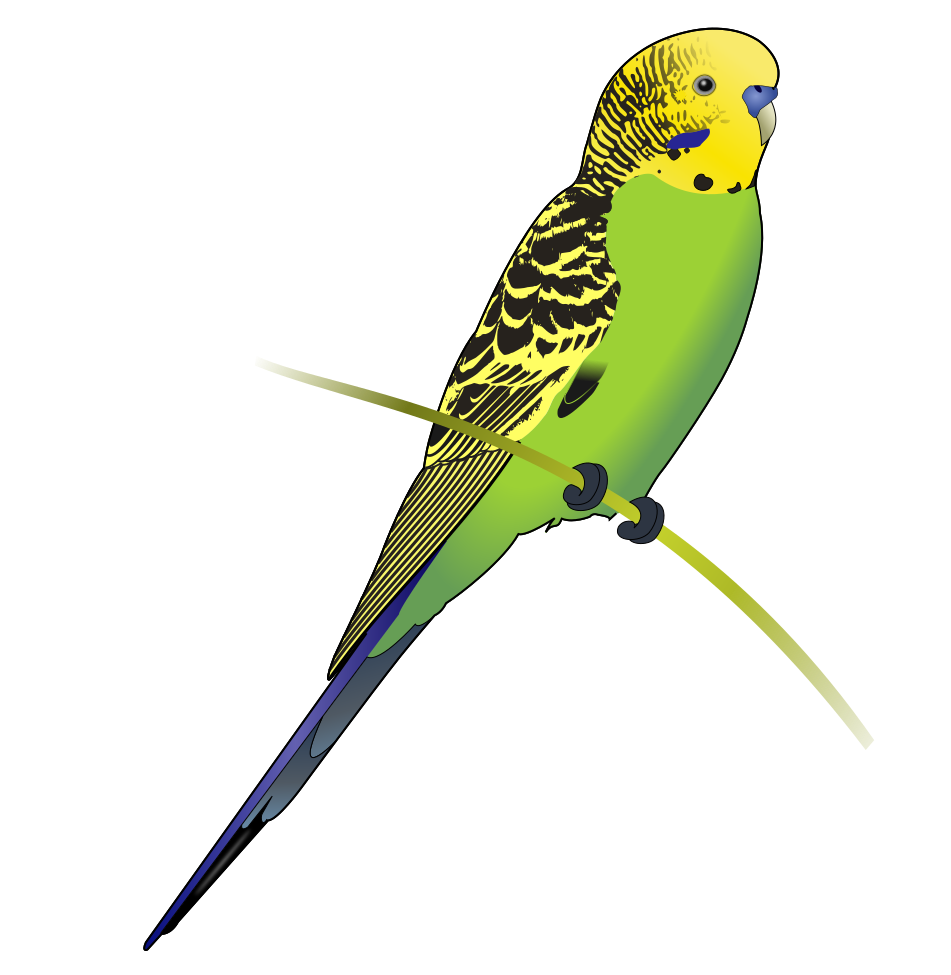
\includegraphics[scale=0.2]{img/others/Budgerigar_diagram.png}
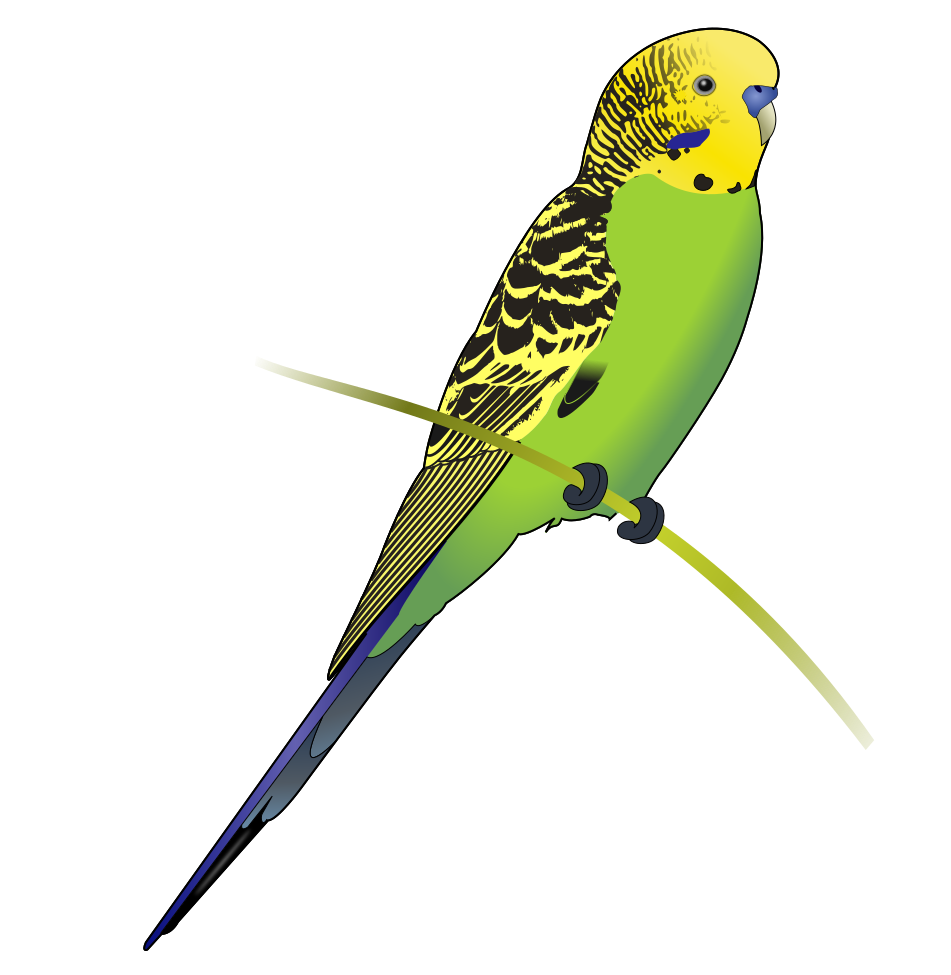
\includegraphics[scale=0.1]{img/others/Budgerigar_diagram.png}
\end{center}

\vspace*{-1cm}

%\vfillLast

%\clearpage

%%%%%%%%%%%%%%%%%%%%%%%%%%%%%%%%%%%%%%%%%%%%%%%%%%%%%%%
%%%%%%%%%%%%%%%%%%%%%%%%%%%%%%%%%%%%%%%%%%%%%%%%%%%%%%%
%%%%%%%%%%%%%%%%%%%%%%%%%%%%%%%%%%%%%%%%%%%%%%%%%%%%%%%

\section{Structure de données et ASCII (6 points)}

\noindent Dans cet exercice, vous allez devoir lire le contenu d'une FAT12 simplifiée pour retrouver le nom et les propriétés de deux fichiers stockés dedans.
Les partitions au format FAT sont généralement séparées en trois parties : le \textit{boot sector}, une \textit{FAT}, et le contenu des fichiers et dossiers.
La partie \textit{FAT} est une simple liste de \textit{direntries}, la structure qui nous intéresse dans cet exercice.

\medskip

\subsection{(2 points) Première étape : lecture d'une structure }

\noindent Une \textit{direntry} correspond à la structure suivante.
Vous devez utiliser le modèle de la structure pour séparer les différents champs et remplir les tableaux suivants avec les valeurs hexadécimales.

\begin{table}[ht!]
  \centering
  \begin{minipage}{0.45\textwidth}
    \centering
% %*   *)
% [style=algorithmique]
\begin{lstlisting}[language=C]
struct direntry {
  char[11] name;
  char     attributes;
  int      first_cluster;
  long     size;
} __attribute__((packed)) \end{lstlisting}
  \end{minipage}
  \hfillx
  \begin{minipage}{0.45\textwidth}
Les types de données font :

\begin{itemize}
\item char : 1 octet (8 bits)
\item int : 2 octets (16 bits)
\item long : 4 octets (32 bits)
\end{itemize}

\textit{Rappel : char[11] correspond à un tableau de 11 cases (de 0 à 10)}
  \end{minipage}
%  \caption{Algorithme de la somme des N premiers entiers}
%  \label{somme-n-premiers-entiers}
\end{table}


%\vspace*{-0.5cm}
\clearpage


\begin{table}[ht!]
  \centering
  \begin{minipage}{0.3\textwidth}
    \centering
% %*   *)
\begin{lstlisting}[style=algorithmique]
direntry 1 :
44 49 4E 4F 53 4F
52 45 4A 50 47 36
00 64 00 00 11 BD

direntry 2 :
47 41 53 4F 4C 49
4E 45 45 31 30 15
00 A3 00 00 07 95
\end{lstlisting}

%\centering{
%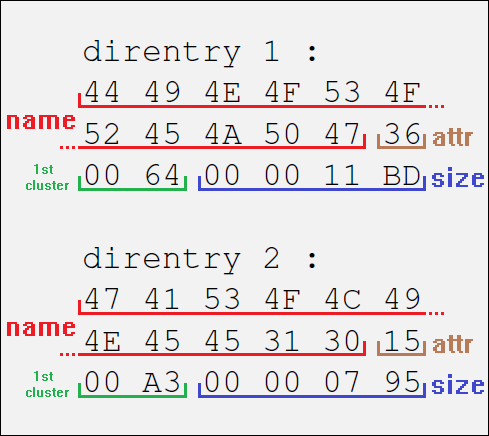
\includegraphics[scale=0.42]{img/Tab_Sujet_underlined.png}
%}

  \end{minipage}
  \hfillx
  \begin{minipage}{0.65\textwidth}
    \centering

\begin{tabular}{ | c |C{0.33cm}|C{0.33cm}|C{0.33cm}|C{0.33cm}|C{0.33cm}|C{0.33cm} | C{0.33cm}|C{0.33cm}|C{0.33cm}|C{0.33cm}|C{0.33cm}|C{0.33cm}| }
\hline
                         & \multicolumn{6}{c|}{direntry[0] (file1)} & \multicolumn{6}{c|}{direntry[1] (file2)} \\
\hline

\multirow[c]{4}{*}[0in]{name} &             & & & & &            &   & & & & & \\
                              &             & & & & &            &   & & & & & \\
\cline{2-13}
                              &             & & & & & \cellcolor{black!65} &   & & & & & \cellcolor{black!65} \\
                              &             & & & & & \cellcolor{black!65} &   & & & & & \cellcolor{black!65} \\
\hline

\multirow[c]{3}{*}[0in]{attributes} & \multicolumn{6}{c|}{ } & \multicolumn{6}{c|}{ } \\
                              & \multicolumn{6}{c|}{ } & \multicolumn{6}{c|}{ } \\
                              & \multicolumn{6}{c|}{ } & \multicolumn{6}{c|}{ } \\
\hline

\multirow[c]{3}{*}[0in]{first\_cluster} & \multicolumn{6}{c|}{ } & \multicolumn{6}{c|}{ } \\
                              & \multicolumn{6}{c|}{ } & \multicolumn{6}{c|}{ } \\
                              & \multicolumn{6}{c|}{ } & \multicolumn{6}{c|}{ } \\
\hline

\multirow[c]{3}{*}[0in]{size} & \multicolumn{6}{c|}{ } & \multicolumn{6}{c|}{ } \\
                              & \multicolumn{6}{c|}{ } & \multicolumn{6}{c|}{ } \\
                              & \multicolumn{6}{c|}{ } & \multicolumn{6}{c|}{ } \\
\hline
\end{tabular}

  \end{minipage}
%  \caption{Algorithme de la somme des N premiers entiers}
%  \label{somme-n-premiers-entiers}
\end{table}


\vspace*{-0.25cm}


\subsection{(2 points) Deuxième étape : conversion des noms }

\noindent À partir de la table ASCII suivante décrivant l'équivalence caractère/valeur décimale, convertissez les noms de fichiers précédemment trouvés de l'hexadécimal vers l'ASCII.

\smallskip

\noindent Concernant les noms de fichiers, la norme FAT12 précise que sur les caractères, les 8 premiers servent à coder le nom du fichier, et les 3 derniers servent à coder l'extension.
Un point est ajouté pour séparer l'extension du nom de fichier.

%\medskip

\begin{center}
%%%%% NOMBRES ET AUTRES
\begin{tabular}{ | l |c|c|c|c|c| c |c|c|c|c|c|c|c|c|c|c| }
\hline
Char & \textbackslash{}n & \textbackslash{}r & { \small \textit{(espace)} } &  - &  . &   & 0 &  1 &  2 &  3 &  4 &  5 &  6 &  7 &  8 &  9 \\
\hline
Dec &         10         &        13         &         32        & 45 & 46 &   & 48 & 49 & 50 & 51 & 52 & 53 & 54 & 55 & 56 & 57 \\
\hline
\end{tabular}

\medskip

%%%%% MAJUSCULES
\begin{tabular}{ | l |c|c|c|c|c|c|c|c|c|c|c|c|c| }
\hline
Char &  A &  B &  C &  D &  E &  F &  G &  H &  I &  J &  K &  L &  M \\
\hline
Dec &  65 & 66 & 67 & 68 & 69 & 70 & 71 & 72 & 73 & 74 & 75 & 76 & 77 \\
\hline
\hline
Char &  N &  O &  P &  Q &  R &  S &  T &  U &  V &  W &  X &  Y &  Z \\
\hline
Dec &  78 & 79 & 80 & 81 & 82 & 83 & 84 & 85 & 86 & 87 & 88 & 89 & 90 \\
\hline
\end{tabular}

\medskip

%%%%% MINUSCULES
\begin{tabular}{ | l |c|c|c|c|c|c|c|c|c|c|c|c|c| }
\hline
Char &  a &  b &  c &  d  &  e  &  f  &  g  &  h  &  i  &  j  &  k  &  l  &  m \\
\hline
Dec &  97 & 98 & 99 & 100 & 101 & 102 & 103 & 104 & 105 & 106 & 107 & 108 & 109 \\
\hline
\hline
Dec &  110 & 111 & 112 & 113 & 114 & 115 & 116 & 117 & 118 & 119 & 120 & 121 & 122 \\
\hline
Char &  n  &  o  &  p  &  q  &  r  &  s  &  t  &  u  &  v  &  w  &  x  &  y  &  z \\
\hline
\end{tabular}

\bigskip

\begin{tabular}{ c   | m{0.45cm} | m{0.45cm} | m{0.45cm} | m{0.45cm} | m{0.45cm} | m{0.45cm} | m{0.45cm} | m{0.45cm} | c | m{0.45cm} | m{0.45cm} | m{0.45cm} | }
\cline{2-9} \cline{11-13}
\multirow[r]{2}{*}[0in]{file1} & & & & & & & & &  \multirow[c]{2}{*}[0in]{.}  & & & \\
 & & & & & & & & &   & & & \\
\cline{2-9} \cline{11-13}
\multirow[r]{2}{*}[0in]{file2} & & & & & & & & &  \multirow[c]{2}{*}[0in]{.}  & & & \\
 & & & & & & & & &   & & & \\
\cline{2-9} \cline{11-13}
\end{tabular}

\end{center}

%\bigskip
\vspace*{-0.25cm}


\subsection{(2 points) Troisième étape : conversion des champs }

\noindent Convertissez maintenant la taille et le numéro du premier cluster de chaque fichier.

%\smallskip
%
%\noindent \textit{Ici, les entiers sont en big endian, c'est-à-dire que les octets sont ordonnés de la même façon que nous représentons les nombres : AUCUNE transformation ou réorganisation n'est nécessaire, vous n'avez qu'à convertir les nombres comme dans la première partie de l'examen.}

\smallskip

\begin{center}
\begin{tabular}{ | c | C{5cm} | C{7.5cm} | }
\hline
 & taille du fichier & numéro du premier cluster \\
\hline
\multirow[c]{3}{*}[0in]{direntry 1 (file1)}
 & & \\
 & & \\
 & & \\
\hline
\multirow[c]{3}{*}[0in]{direntry 2 (file2)}
 & & \\
 & & \\
 & & \\
\hline
\end{tabular}
\end{center}


%\bigskip
\clearpage


%%%%%%%%%%%%%%%%%%%%%%%%%%%%%%%%%%%%%%%%%%%%%%%%%%%%%%%
%%%%%%%%%%%%%%%%%%%%%%%%%%%%%%%%%%%%%%%%%%%%%%%%%%%%%%%
%%%%%%%%%%%%%%%%%%%%%%%%%%%%%%%%%%%%%%%%%%%%%%%%%%%%%%%

% Circuits logiques
\section{Circuits logiques (4 points)}

\subsection{(1 point) \'Ecrivez la formule associée à ce schéma : }

\begin{figure}[ht!]
\centering{
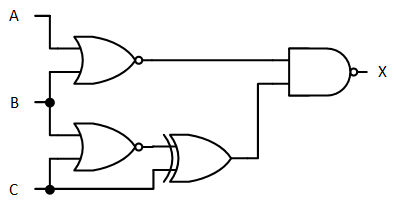
\includegraphics[scale=2]{./img/circuit_logique.png}
}
\end{figure}

% X  =  ( A NOR B )  NAND  ( (B NOR C) XOR C )
% $ \text{X} \; = \; \overline{ ( \overline{\text{A} \, + \, \text{B}} ) \; \cdot \; ( \; ( \overline{\text{B} \, + \, \text{C}} ) \; \oplus \; \text{C} ) } $

\bigskip
\bigskip
%\bigskip
%\bigskip

\bigskip


\subsection{(1 point) Remplissez la table de vérité de la formule précédente : }

%\bigskip
\medskip

%\begin{center}
%\begin{tabular}{|c|c|c||c|}
%\hline
%\cellcolor{black!15} \textbf{A} & \cellcolor{black!15} \textbf{B} & \cellcolor{black!15} \textbf{C} &  \cellcolor{black!15} \textbf{X} \\
%\hline
%\hline
%0 & 0 & 0  &  \cellcolor{black!15} 0 \\ \hline
%0 & 0 & 1  &  \cellcolor{black!15} 0 \\ \hline
%0 & 1 & 0  &  \cellcolor{black!15} 1 \\ \hline
%0 & 1 & 1  &  \cellcolor{black!15} 1 \\ \hline
%1 & 0 & 0  &  \cellcolor{black!15} 1 \\ \hline
%1 & 0 & 1  &  \cellcolor{black!15} 1 \\ \hline
%1 & 1 & 0  &  \cellcolor{black!15} 1 \\ \hline
%1 & 1 & 1  &  \cellcolor{black!15} 1 \\ \hline
%\end{tabular}
%\end{center}

\begin{center}
\begin{tabular}{|C{0.75cm}|C{0.75cm}|C{0.75cm} | C{0.75cm}|}
\hline
\cellcolor{black!15} & \cellcolor{black!15} & \cellcolor{black!15}  &  \cellcolor{black!15} \\
\cellcolor{black!15} & \cellcolor{black!15} & \cellcolor{black!15}  &  \cellcolor{black!15} \\
\hline
 & &   & \cellcolor{black!15} \\
 & &   & \cellcolor{black!15} \\ \hline
 & &   & \cellcolor{black!15} \\
 & &   & \cellcolor{black!15} \\ \hline
 & &   & \cellcolor{black!15} \\
 & &   & \cellcolor{black!15} \\ \hline
 & &   & \cellcolor{black!15} \\
 & &   & \cellcolor{black!15} \\ \hline
 & &   & \cellcolor{black!15} \\
 & &   & \cellcolor{black!15} \\ \hline
 & &   & \cellcolor{black!15} \\
 & &   & \cellcolor{black!15} \\ \hline
 & &   & \cellcolor{black!15} \\
 & &   & \cellcolor{black!15} \\ \hline
 & &   & \cellcolor{black!15} \\
 & &   & \cellcolor{black!15} \\ \hline
\end{tabular}
\end{center}


%\medskip
\smallskip

\subsection{(2 points) Remplissez le tableau de Karnaugh, formez les groupes, et déduisez-en la formule réduite : }

%\bigskip

\begin{table}[!ht]
  \centering
  \begin{minipage}{0.08\textwidth}
    \centering

\vfillFirst

\_\_

% A

\vfillLast

  \end{minipage}
  \hfillx
  \begin{minipage}{0.37\textwidth}
    \centering

\begin{center}

\_\_  \_\_

% BC

\medskip

%\begin{tabular}{|C{0.75cm} || C{0.75cm}|C{0.75cm}|C{0.75cm}|C{0.75cm}|}
%\hline
%\cellcolor{black!65}  &  \cellcolor{black!15} 00 & \cellcolor{black!15} 01 & %\cellcolor{black!15} 11 & \cellcolor{black!15} 10 \\
%\hline
%\hline
%\cellcolor{black!15} 0 &  0 & 0 & 1 & 1 \\ \hline
%\cellcolor{black!15} 1 &  1 & 1 & 1 & 1 \\ \hline
%\end{tabular}

\begin{tabular}{|C{0.75cm} | C{0.75cm}|C{0.75cm}|C{0.75cm}|C{0.75cm}|}
\hline
\cellcolor{black!65}  &  \cellcolor{black!15} & \cellcolor{black!15} & \cellcolor{black!15} & \cellcolor{black!15} \\
\cellcolor{black!65}  &  \cellcolor{black!15} & \cellcolor{black!15} & \cellcolor{black!15} & \cellcolor{black!15} \\
\hline
\cellcolor{black!15}  &  & & & \\
\cellcolor{black!15}  &  & & & \\ \hline
\cellcolor{black!15}  &  & & & \\
\cellcolor{black!15}  &  & & & \\ \hline
\end{tabular}

\end{center}

  \end{minipage}
  \hfillx
  \begin{minipage}{0.55\textwidth}
    \centering

Formule réduite :

\vspace{2cm}

\vfillFirst

\phantom{42}

% $ X = B \; + \; A $

\vfillLast

  \end{minipage}
\end{table}

%%%%%%%%%%%%%%%%%%%%%%%%%%%%%%%%%%%%%%%%%%%%%%%%%%%%%%%%%%%%%%%%%%%%%%%%%%%%%

%\vfillFirst
%
%\begin{center}
%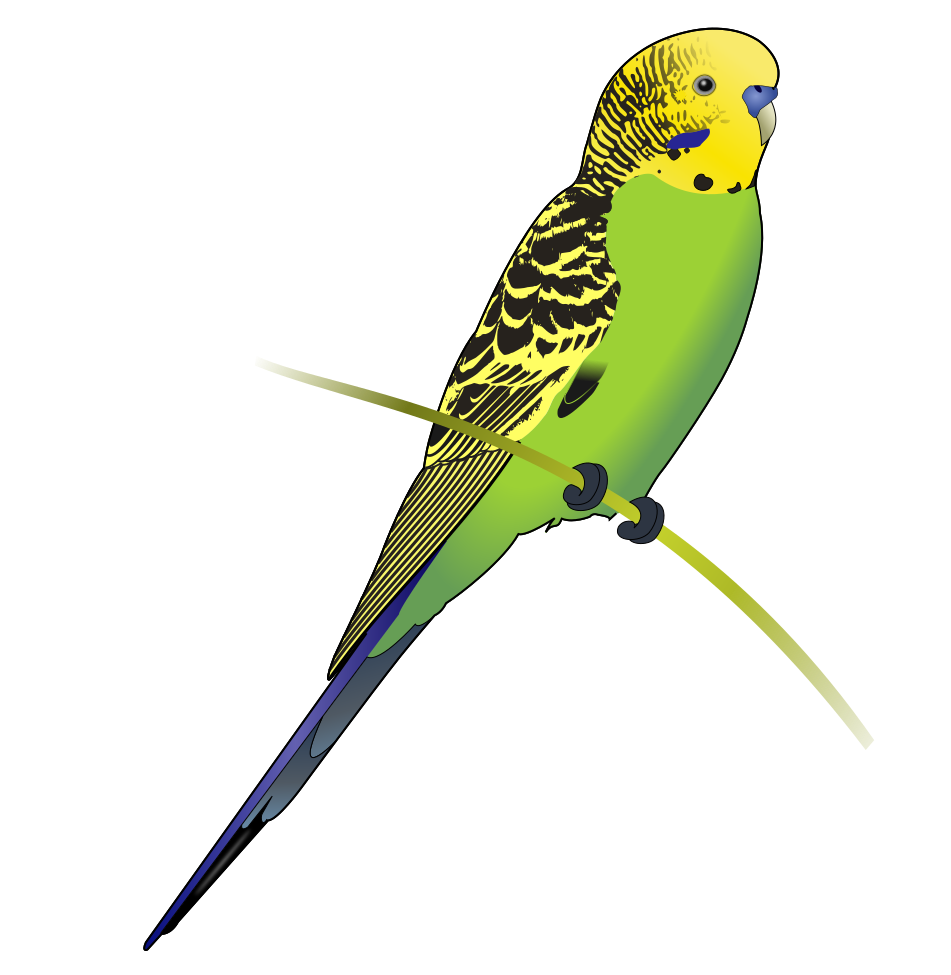
\includegraphics[scale=0.2]{img/others/Budgerigar_diagram.png}
%\end{center}
%
%\vfillLast

%\clearpage

%
%%\thispagestyle{empty}
%
%\vfillFirst
%
%\begin{center}
%
%\begin{LARGE}
%\textbf{SUJET RATTRAPAGE}
%
%\bigskip
%
%\textbf{\MakeUppercase{\TitreMatiere}}
%\end{LARGE}
%
%\end{center}
%
%\vfillLast

\end{document}
